\documentclass[a4paper]{article}

\usepackage[portuguese]{babel}
\usepackage[utf8]{inputenc}
\usepackage[T1]{fontenc}
\usepackage{graphicx}
\usepackage{caption}
\usepackage{anysize}
\usepackage{amsmath}

\usepackage{hyperref}
\hypersetup{
	pdftitle = {CAD - TP2}
	,pdfauthor = {João Ferreira \& José Ribeiro Departamento de Engenharia Informática Universidade De Coimbra \texttt{jpbat@student.dei.uc.pt |  jbaia@student.dei.uc.pt}}
	,pdfborder = {0 0 0}
}

\title{Computação de Alto Desempenho - Trabalho Prático 2}
\author{João Ferreira \& José Ribeiro\\
		Departamento de Engenharia Informática\\
		Universidade de Coimbra\\
		\texttt{jpbat@student.dei.uc.pt | jbaia@student.dei.uc.pt}\\
		\texttt{2009113274 | 2008112181}}
\date{Junho 2013}

\marginsize{3.5cm}{3.5cm}{3cm}{3cm}

\begin{document}
\maketitle

\clearpage

\tableofcontents
\clearpage

\setlength{\parindent}{1cm}
\setlength{\parskip}{0.3cm}

\section{Introdução}
\indent \indent Tal como foi referido no relatório anterior, é cada vez mais díficil aumentar a frequência dos processadores, pelo que se verificou um aumento do número de processadores por computador. No entanto como seria fácil de prever também este aumento tem uma barreira, pelo que existiu a necessidade de apostar em computação distribuida.

Assim aparece o conceito de cluster, um aglomerado de computadores que estão ligados a um switch de alta velocidade o que lhes permite fazer computação distribuida através de, por exemplo, passagem de mensagens entre eles.

Assim aparece a biblioteca \textit{Message Passing Interface}, que nos foi apresentada pelo docente nas aulas teóricas e que vai ser por nós utilizada neste projecto.

Tal como no relatório anterior vai ser explicado o algoritmo utilizado, passando-se depois à análise dos resultados dos testes efectuados.
\clearpage


\section{Ambiente de Testes}
\indent \indent Os testes foram executados nos servidores disponibilizados pelo professor, sendo que pelo que nos foi possível constatar estas são as especificações técnicas de cada um deles:
\begin{description}
	\item [Processador] Intel(R) Xeon(R) CPU E5405 @ 2.00GHz, que possui 2 cores e 12MB de L2 Cache.
	\item [Memória RAM] 3.7GB.
	\item [Sistema Operativo] CentOS 6.3.
\end{description}

\section{Abordagens}
\indent \indent Uma vez que no primeiro projecto criámos aquilo que achámos ser a melhor solução possível para resolver o problema, a nossa solução passa por correr a nossa versão 1.0 do projecto em cada uma das máquinas, sendo que em cada uma dessas máquinas o projecto vai estar a fazer \textit{matching} às transacções que lhe forem atribuidas e depois enviar os \textit{matches} para o master, que tem como função juntar as respostas de todos os \textit{workers} e escrever para ficheiro.

Após isto foi necessário fazer \textit{fine tune} a alguns valores, como por exemplo qual o tamanho ideal do \textit{buffer} de envio em cada uma das máquinas, ou qual a dimensão do \textit{batch} de trabalhos que minimizava o tempo em que os processadores ficavam parados. Este processo nem sempre se verificou ser fácil, uma vez que por vezes em execuções consecutivas com os mesmos valores chegavam a haver variações de 2 segundos nos tempos de execução (25\%) o que obrigava a um grande número de execuções até que se chegasse a qualquer tipo de conclusão sobre a possível modificação de um valor.

Durante todos os testes efectuados verificou-se com o auxílio de ferramentas como o \textit{htop}, se existiriam mais alunos a utilizar os servidores, e o nível de ocupação dos vários processadores das máquinas utilizadas, de modo a que houvesse certezas sobre a validade dos resultados.
\begin{figure}[h]
	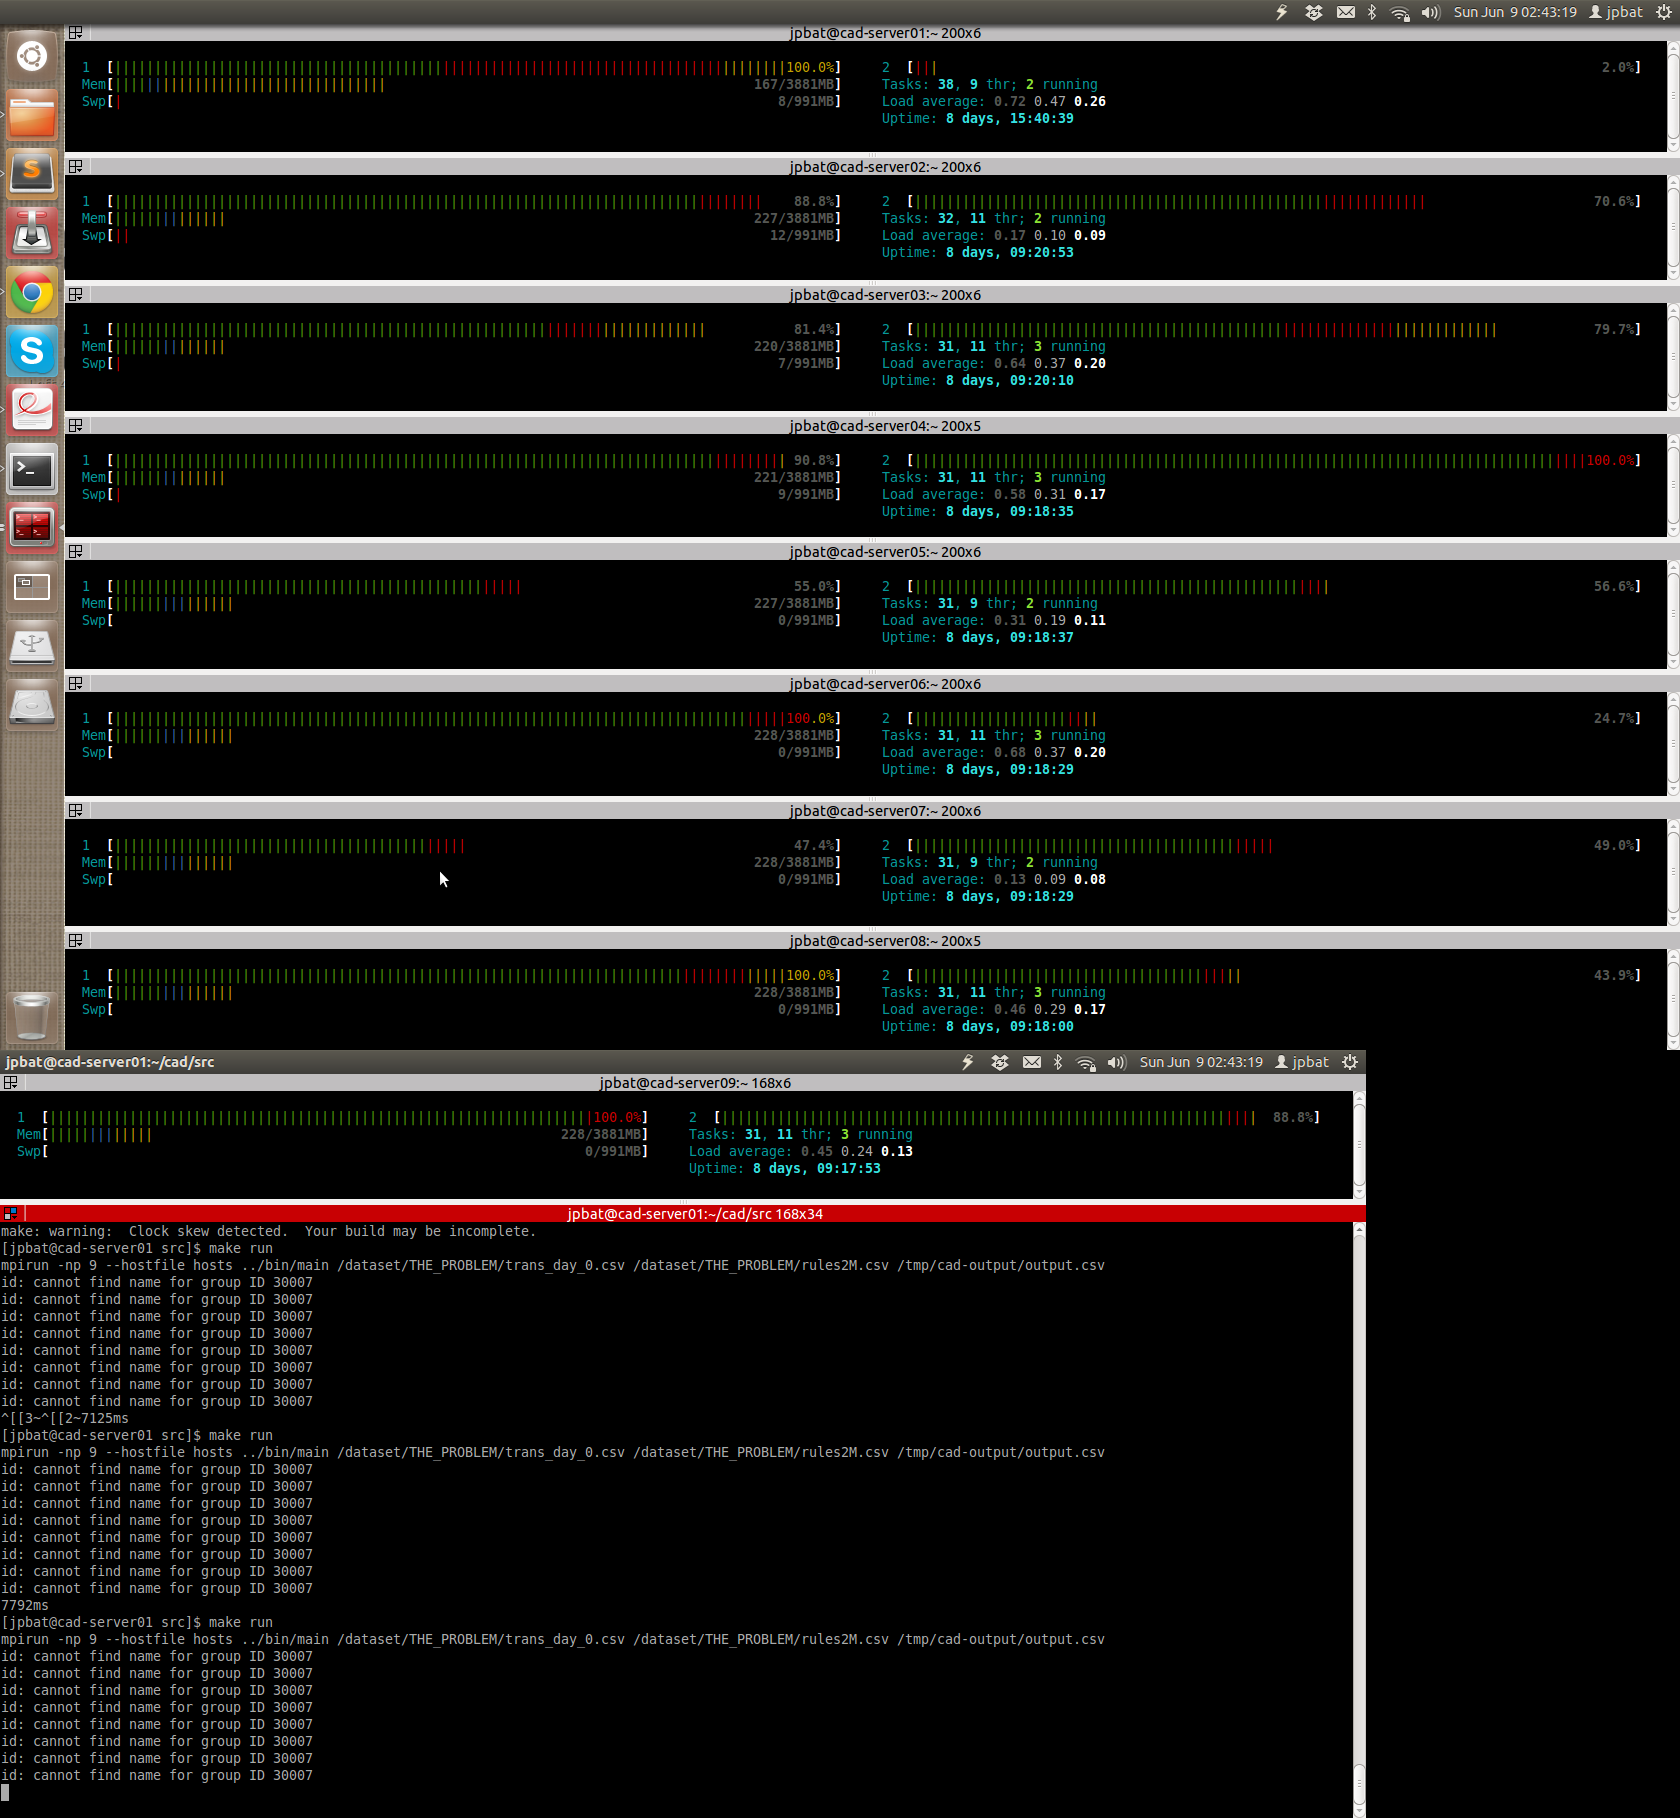
\includegraphics[keepaspectratio=true, width=0.4\textheight]{imgs/ocupacao.png}
	\caption{Monitorização do nível de ocupação dos CPUs.}
\end{figure}
\clearpage


\section{Resultados}
\indent \indent TODO:GRÁFICO COM VARIAÇÃO DE TEMPO E NUMERO DE MAQUINAS ENTRE 2 E 9!!!
\clearpage


\section{Conclusão}
\indent \indent Com o fim do projecto, já depois de termos reflectido sobre todos os dados que foram recolhidos, chega por fim a altura em que se tiram conclusões.


\clearpage



\end{document}
